\section{Results and Analysis}\label{sec:results}

\subsection{Comparison of Clustering Scores and Runtime}\label{sec:silhouette-results}

The silhouette scores of the three methods and the measured end-to-end runtimes of the two deep workflows are summarized in Table~\ref{tab:silhouette}. All methods use the same six-channel particle data, a 32-dimensional representation, and five clusters. Evaluation is performed on the same subset of 10,000 particles.

\begin{table}[htbp]
\centering\small
\caption{Silhouette scores and end-to-end runtimes. Scores use Euclidean distance on the same sample of 10,000 particles, within each method's own 32-dimensional representation space. Runtimes were measured for 12,800 particles on an NVIDIA RTX PRO 6000 Blackwell Server Edition GPU and include preprocessing, autoencoder pretraining, 350 refinement epochs, evaluation, and figure generation. The PCA baseline runtime was not measured.}\label{tab:silhouette}
\begin{tabularx}{\linewidth}{@{}p{0.21\linewidth}Y c c r r@{}}
\toprule
\textbf{Method} & \textbf{Evaluation space} & \textbf{\shortstack{Latent\\dim.}} & \textbf{$K$} & \textbf{Silhouette} & \textbf{\shortstack{Runtime\\(s)}} \\
\midrule
PCA + K-means & PCA representation & 32 & 5 & 0.29957 & --- \\
1D CNN + DEC & Time-series latent space & 32 & 5 & 0.79637 & 405.19 \\
\shortstack[l]{Spectrogram CNN\\+ DEC} & Spectrogram latent space & 32 & 5 & 0.87985 & 524.62 \\
\bottomrule
\end{tabularx}
\end{table}

PCA + K-means achieves a silhouette score of 0.29957. It obtains this result by applying a linear projection to compress the spectrogram input before carrying out the clustering, and thus provides a baseline for comparison with the deep learning methods.

The 1D CNN + DEC method, by dealing directly with multichannel time series, attains a silhouette score of 0.79637. The fact that this score is higher shows that, with the current setup, the combination of one-dimensional convolutional representation learning and clustering refinement results in a representation that has a higher internal clustering score than the PCA baseline.

The version that uses Spectrogram CNN together with DEC attains the highest silhouette score, which is 0.87985 and is about 0.08348 higher than the 1D result. Hence, with respect to the dataset and training settings examined in this case, the spectrogram-based approach achieves the best score for both within-cluster cohesion and between-cluster separation in its final representation space.

\subsection{Computational Cost and Scalability}

On the NVIDIA RTX PRO 6000 Blackwell Server Edition GPU, end-to-end runtimes for 12,800 particles were 524.62~s for the spectrogram-based workflow and 405.19~s for the 1D time-series workflow. These measurements include preprocessing, autoencoder pretraining, 350 epochs of clustering refinement, evaluation, and figure generation. In the future, using the spectrogram-based workflow on larger PIC datasets with one to ten million tracked particles would need considerably more computational resources. Assuming approximately linear scaling with the number of particles and unchanged per-particle input dimensions and training settings, the estimated run time would be around 11.4 hours for one million particles and 4.7 days for ten million particles on the same hardware. These estimates give a first indication of the computational cost; actual deployment at this scale would also demand efficient data loading and memory management.

\subsection{Training Process of the Spectrogram Method}

The training curves provide supplementary information about the optimization of the main method. Figure~\ref{fig:training} shows the training and validation reconstruction losses during autoencoder pretraining, the loss components during DEC refinement, and the latent-space silhouette monitored during refinement.

\begin{figure}[htbp]
\centering
\begin{subfigure}[t]{0.48\linewidth}
\centering
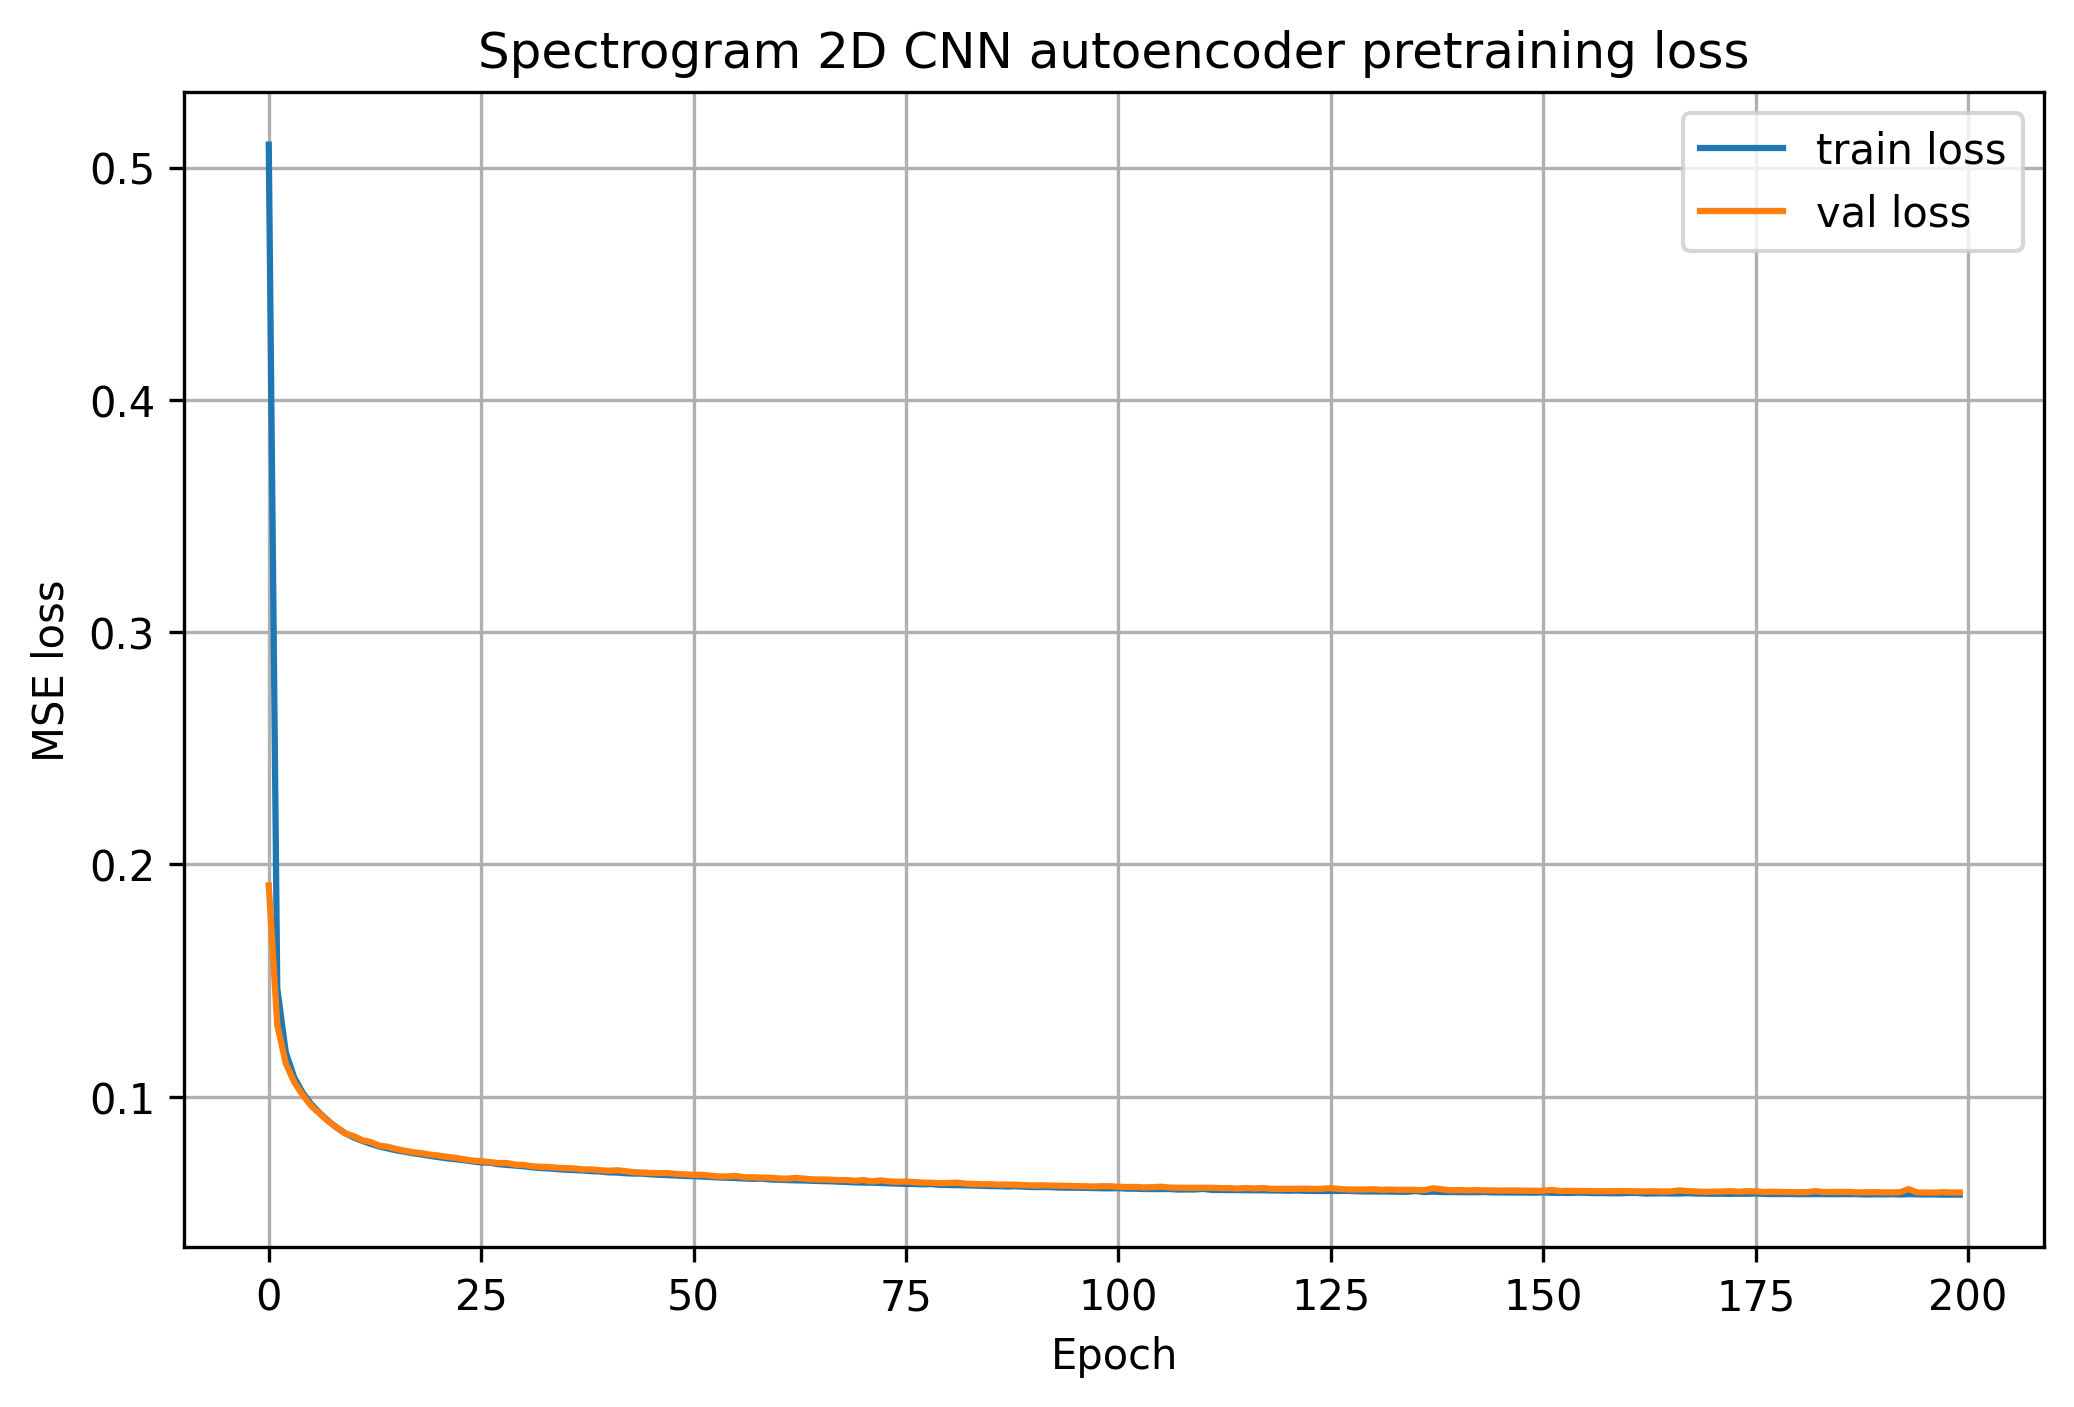
\includegraphics[width=\linewidth]{figures/ae-pretraining-loss.png}
\caption{Pretraining reconstruction losses.}
\end{subfigure}\hfill
\begin{subfigure}[t]{0.48\linewidth}
\centering
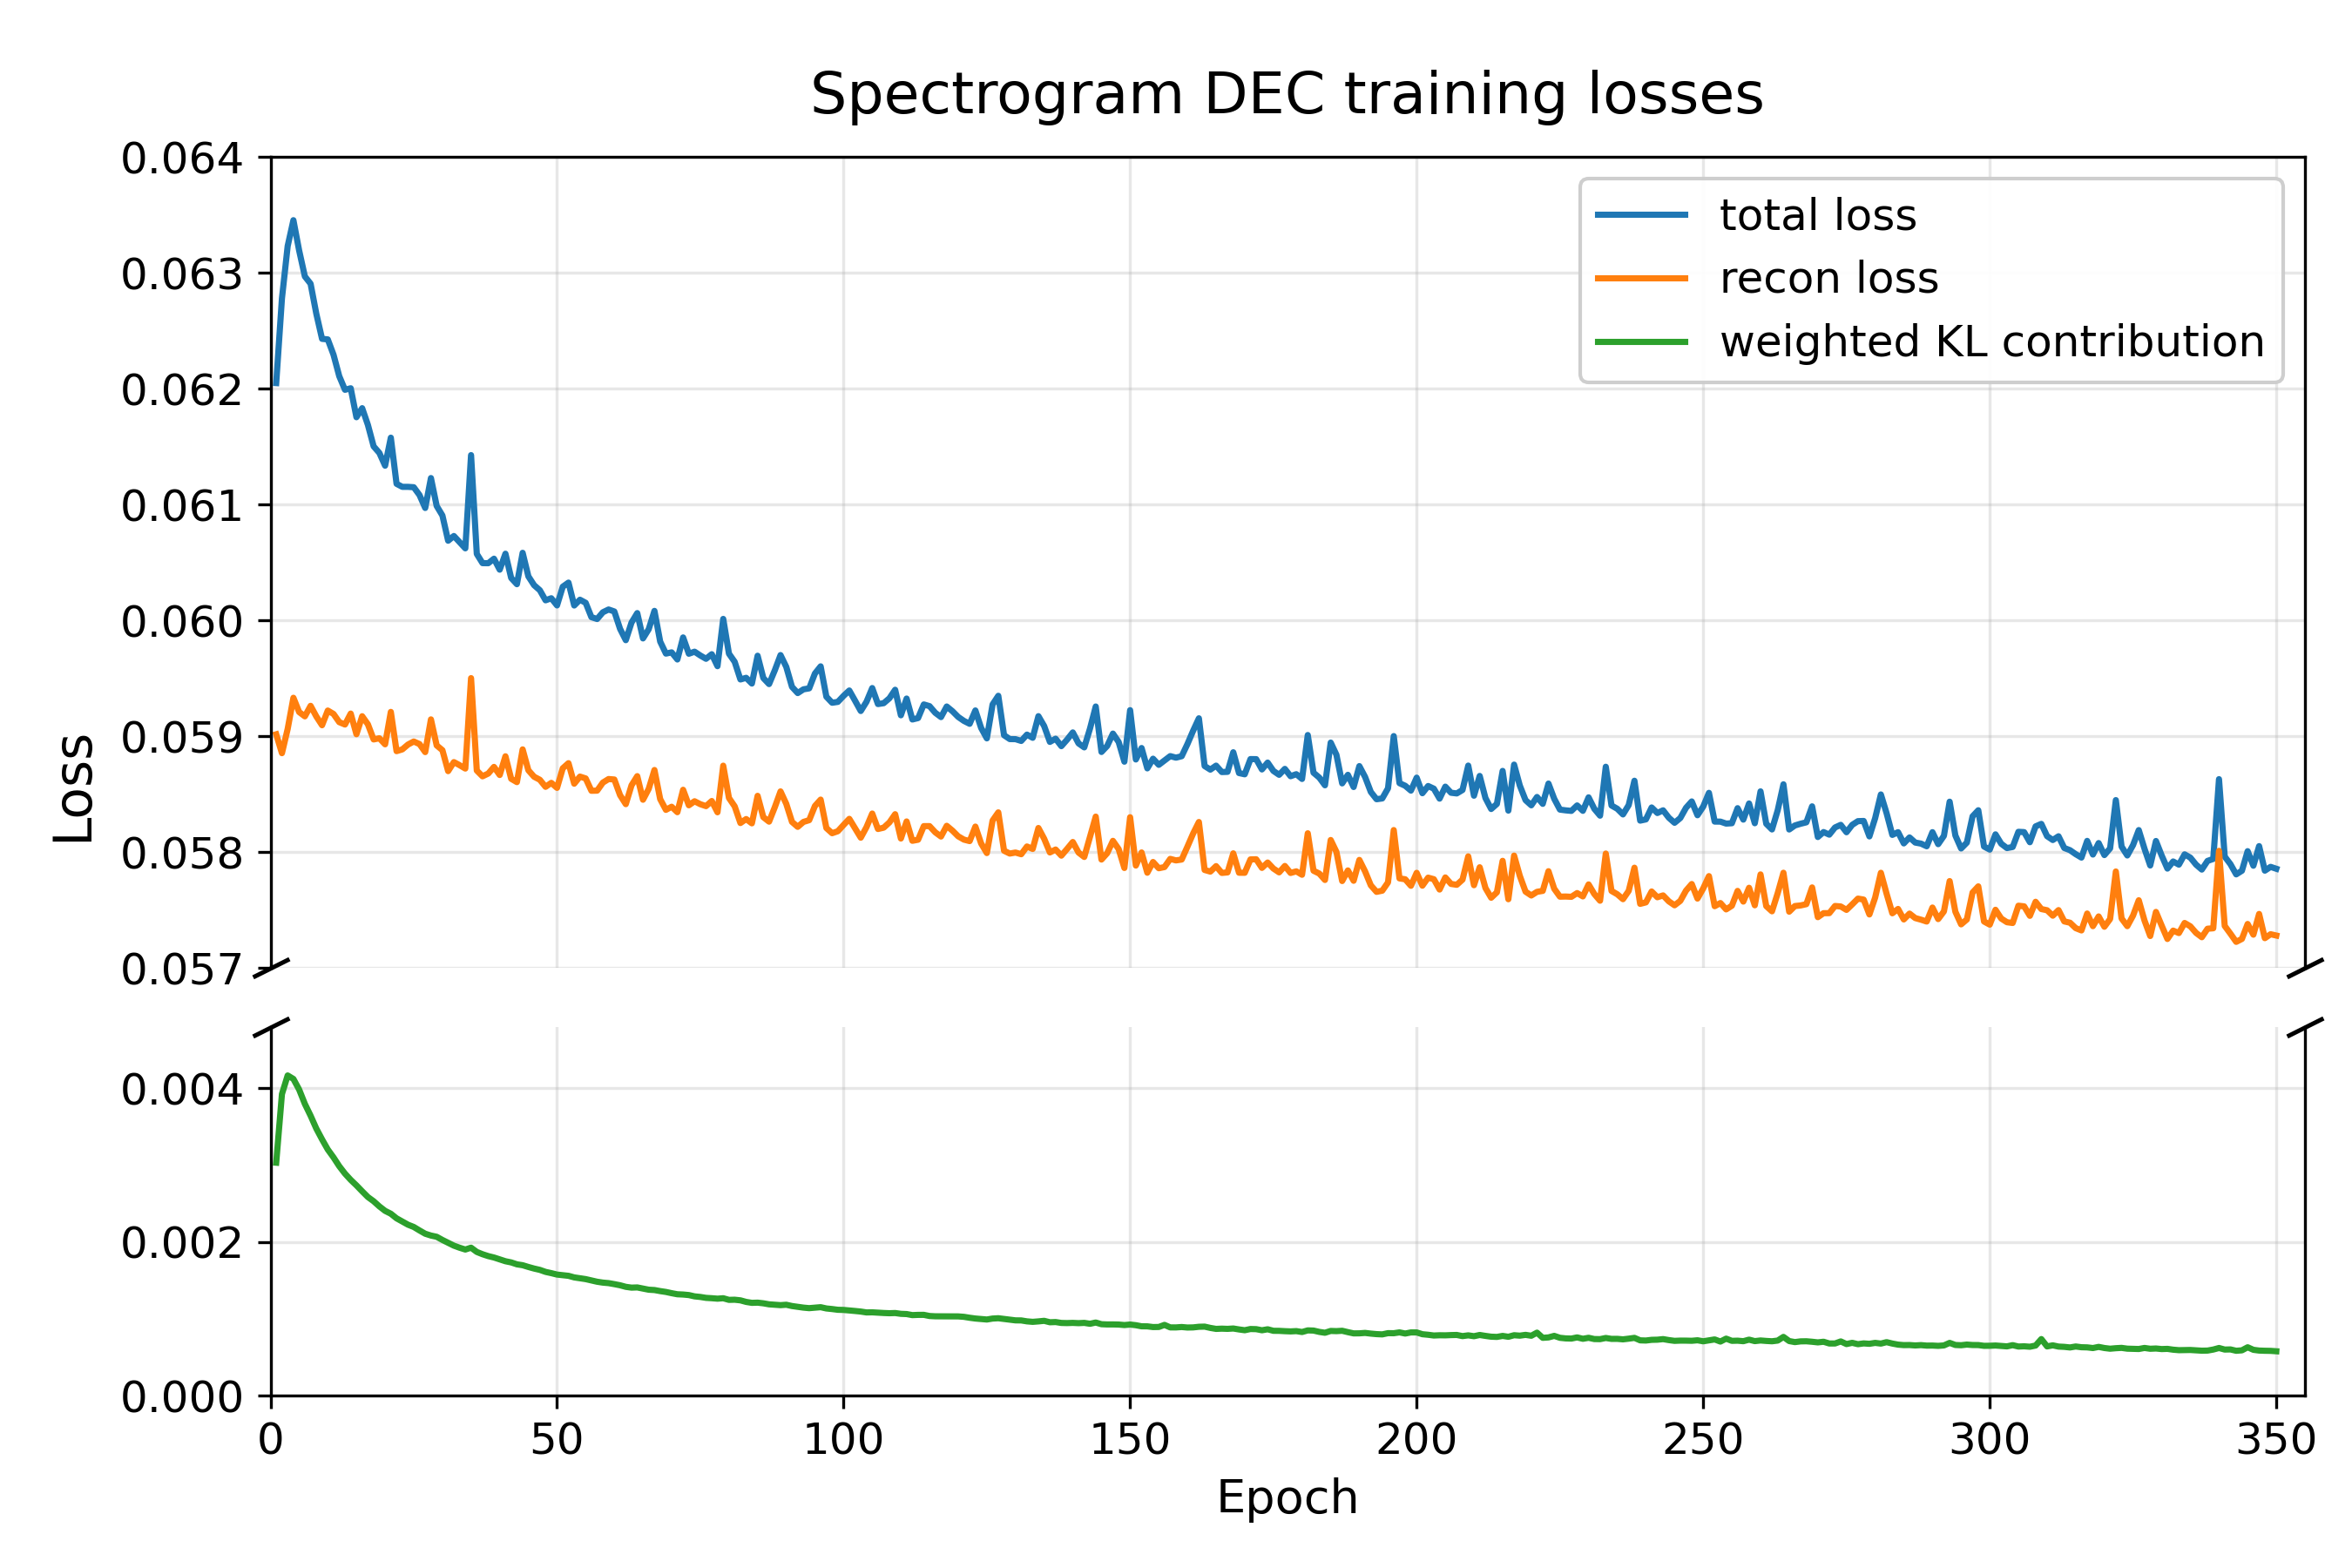
\includegraphics[width=\linewidth]{figures/dec-training-loss-zoomed.png}
\caption{DEC refinement losses with a broken vertical axis.}
\end{subfigure}
\par\medskip
\begin{subfigure}[t]{0.48\linewidth}
\centering
\figureasset[\linewidth]{figures/dec-silhouette.png}{Latent-space silhouette}
\caption{Latent-space silhouette.}
\end{subfigure}
\caption[Training and monitoring diagnostics for the spectrogram method]{Training and monitoring diagnostics for the spectrogram method. (a) Training and validation reconstruction losses during autoencoder pretraining. (b) Total loss, reconstruction loss, and the weighted KL contribution during DEC refinement. (c) Latent-space silhouette during refinement. Training-time silhouette monitoring uses a fixed sample of 5,000 particles, while final evaluation uses 10,000 particles.}
\label{fig:training}
\end{figure}

In the early epochs of pretraining, the training and validation reconstruction losses drop quickly and then fall off more slowly, staying nearly the same for the majority of the training process. These losses are used to monitor learning and to select the autoencoder weights for the clustering phase. DEC then jointly optimizes both the reconstruction and clustering objectives, updating both the representation and the cluster centers. After this initial transient period, the total loss and the weighted KL term both decrease, while the reconstruction loss changes more slowly. The monitored latent-space silhouette rises as the process is refined.

The clustering term is defined as the KL divergence summed over the current minibatch and weighted by \(5\times10^{-4}\). Since the loss plot displays the weighted KL contribution, the numerical size of this component can be compared with that of the reconstruction term. However, the coefficient must be interpreted in light of the loss-reduction convention, since its magnitude alone does not indicate the extent to which clustering optimization affects the result.

The main method carries out 350 DEC training epochs. During training, the silhouette score uses a fixed sample of 5,000 particles, while the final evaluation uses 10,000 particles. As a result, the scores obtained during monitoring and at the end need not be the same. The final evaluation also uses the selected model weights, and these weights do not necessarily correspond to the last training epoch.

These curves describe the optimization and model-selection process. The comparison between methods remains based on the final scores obtained using the common evaluation sample in Section~\ref{sec:silhouette-results}.

\FloatBarrier
\subsection{Reconstruction of the Six-Channel Spectrograms}

To show how the autoencoder reconstructs data, the input and reconstructed spectrograms for a particular particle are displayed side by side for all six channels. The reconstruction uses the pretrained model with the lowest validation reconstruction loss. Figure~\ref{fig:reconstruction} shows this comparison.

\begin{figure}[htbp]
\centering
\figureasset[0.83\linewidth]{figures/reconstruction.png}{Six-channel spectrogram reconstruction}
\caption[Six-channel spectrogram reconstruction]{Six-channel spectrogram reconstruction by the pretrained autoencoder. The left column shows the input spectrograms of a selected particle, and the right column shows the corresponding reconstructions. Rows represent the \(x\), \(p_x\), \(p_y\), \(E_x\), \(E_y\), and \(B_z\) channels, respectively. Reconstructions are obtained from the pretrained model with the lowest validation reconstruction loss.}\label{fig:reconstruction}
\end{figure}

The six channels describe particle position, momentum components, and local electromagnetic field components. The paired display provides a visual comparison between the input and reconstruction for each channel, so that differences in spectral distributions and local details can be examined.

Reconstruction and silhouette evaluate different aspects of the model. Reconstruction measures the autoencoder's ability to reproduce its input, while silhouette reflects the grouping structure in the chosen representation space. Reconstruction is therefore employed as a supplementary diagnostic rather than as a direct criterion for assessing clustering quality.

\subsection{Visualization of the Final Clustering}

The final 32-dimensional representations of the spectrogram method are projected into two dimensions using PCA and t-SNE. Particles are colored according to their final cluster assignments. Figure~\ref{fig:latent-projections} shows both projections.

\begin{figure}[htbp]
\centering
\begin{subfigure}[t]{0.49\linewidth}
\centering
\figureasset[\linewidth]{figures/latent-pca.png}{PCA projection}
\caption{PCA projection.}
\end{subfigure}\hfill
\begin{subfigure}[t]{0.49\linewidth}
\centering
\figureasset[\linewidth]{figures/latent-tsne.png}{t-SNE projection}
\caption{t-SNE projection.}
\end{subfigure}
\caption[Two-dimensional projections of the final latent representations]{Two-dimensional visualization of the final spectrogram CNN + DEC representations. Colors indicate the five final cluster assignments. Clustering and silhouette evaluation are performed in the 32-dimensional latent space; the two-dimensional projections are used only for visualization.}
\label{fig:latent-projections}
\end{figure}

The PCA projection provides a linear view of the latent distribution, and the t-SNE projection offers a supplementary visualization of local neighborhood relationships. Both plots use the previously obtained final labels; clustering is not repeated in the two-dimensional coordinates.

These visualizations allow a qualitative examination of how the clusters are distributed. Because a two-dimensional projection retains only part of the high-dimensional structure, visual distances do not directly correspond to distances in the full latent space. The silhouette score was calculated using all 32 latent dimensions.

\subsection{Final Cluster Sizes}

The main method partitions the 12,800 particles into five nonempty clusters. Their sizes and proportions are listed in Table~\ref{tab:cluster-sizes} in Appendix~\ref{app:clusters}.

The largest group consists of 3,884 particles (30.34\% of the dataset), and the smallest group has 1,818 particles (14.20\%). Each of the five clusters includes a large number of particles, with no empty clusters and no clusters with only a small number of particles.

The cluster-size distribution supplements the silhouette evaluation by describing how particles are distributed among the groups. Cluster size alone does not establish the correctness of a partition, nor does the clustering objective require equally sized groups.